\documentclass[10pt,letterpaper]{report}
\usepackage[latin1]{inputenc}
\usepackage{amsmath}
\usepackage{amsfonts}
\usepackage{amssymb}
\usepackage{graphicx}
%\usepackage{blindtext}
\usepackage{listings}
\usepackage{enumerate}
%\usepackage{enumitem}
\usepackage{hyperref}
%\usepackage{cancel}
%\usepackage{color,soul}
%\usepackage{multirow}
\usepackage{float}
\usepackage[left=1.00in, right=1.00in, top=1.00in, bottom=1.00in]{geometry}
\author{Derek Lontine, Stuart Childs, Alex Bailey}
\title{AFEM: Axisymmetric Project Verification Tests}

\usepackage{color}
 
\definecolor{codegreen}{rgb}{0,0.6,0}
\definecolor{codegray}{rgb}{0.5,0.5,0.5}
\definecolor{codepurple}{rgb}{0.58,0,0.82}
\definecolor{backcolour}{rgb}{0.95,0.95,0.92}
 
\lstdefinestyle{mystyle}{
    backgroundcolor=\color{backcolour},   
    commentstyle=\color{codegreen},
    keywordstyle=\color{magenta},
    numberstyle=\tiny\color{codegray},
    stringstyle=\color{codepurple},
    basicstyle=\footnotesize,
    breakatwhitespace=false,         
    breaklines=true,                 
    captionpos=b,                    
    keepspaces=true,                 
    numbers=left,                    
    numbersep=5pt,                  
    showspaces=false,                
    showstringspaces=false,
    showtabs=false,                  
    tabsize=2
}
\lstset{style=mystyle}

%Tensor notation undertildes
%\usepackage{stackengine} 
%\stackMath 
\newcommand\tenq[2][1]{ \def\useanchorwidth{T} \ifnum#1>1 \stackunder[0pt]{\tenq[\numexpr#1-1\relax]{#2}}{\scriptscriptstyle\sim} \else \stackunder[1pt]{#2}{\scriptscriptstyle\sim} \fi } 



\numberwithin{equation}{chapter}


\usepackage{empheq}
 
% Command "alignedbox{}{}" for a box within an align environment
% Source: http://www.latex-community.org/forum/viewtopic.php?f=46&t=8144
\newlength\dlf  % Define a new measure, dlf
\newcommand\alignedbox[2]{
% Argument #1 = before & if there were no box (lhs)
% Argument #2 = after & if there were no box (rhs)
&  % Alignment sign of the line
{
\settowidth\dlf{$\displaystyle #1$}  
    % The width of \dlf is the width of the lhs, with a displaystyle font
\addtolength\dlf{\fboxsep+\fboxrule}  
    % Add to it the distance to the box, and the width of the line of the box
\hspace{-\dlf}  
    % Move everything dlf units to the left, so that & #1 #2 is aligned under #1 & #2
\boxed{#1 #2}
    % Put a box around lhs and rhs
}
}


\begin{document}
%\maketitle
%
%\chapter{Introduction}
%This document compiles several types of closed form verification tests that can be compared against in the finite element solutions. It provides several examples and the closed form solutions for these examples. 
%
%\chapter{Example 1: Uniaxial Stress on Bar}
%This example performs a simple uniaxial stress test on an axisymmetric bar. An example of a mesh that could be applied to this problem 
%
%\section{Closed form solution}
%
%\chapter{Example 2: Pressure Applied to Simply Supported Circular Plate}
%
%%http://www.roymech.co.uk/Useful_Tables/Mechanics/Plates.html
%
%\begin{figure}[!h]
%\centering
%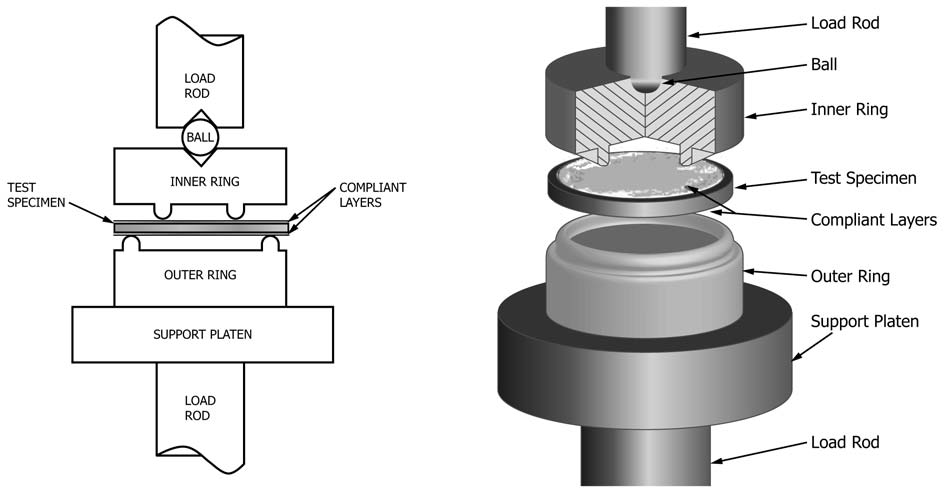
\includegraphics[width=0.7\linewidth]{./BD_3}
%\caption{}
%\label{fig:BD_3}
%\end{figure}
%\begin{figure}[!h]
%\centering
%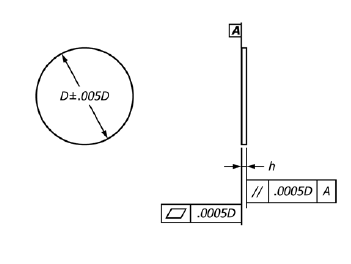
\includegraphics[width=0.7\linewidth]{./BD_2}
%\caption{}
%\label{fig:BD_2}
%\end{figure}
%\begin{figure}[!h]
%\centering
%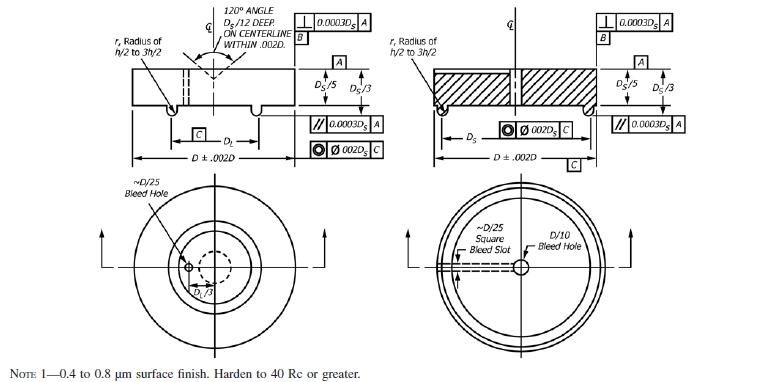
\includegraphics[width=0.7\linewidth]{./BD_1}
%\caption{}
%\label{fig:BD_1}
%\end{figure}
%\begin{figure}[!h]
%\centering
%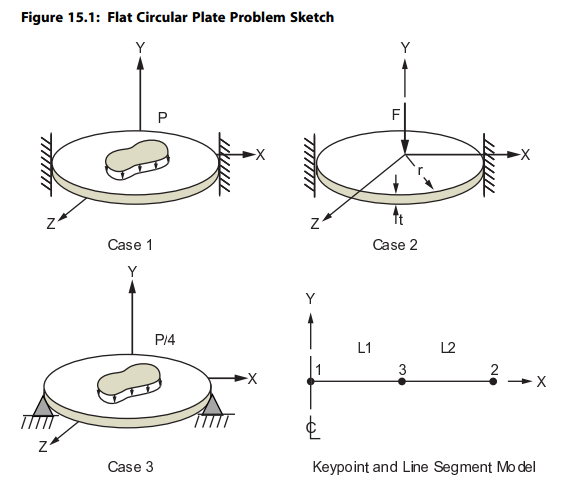
\includegraphics[width=0.7\linewidth]{./BD_4}
%\caption{}
%\label{fig:BD_4}
%\end{figure}
%
%
%\section{Closed form solution}
%
%See Ansys Verification Problems p55
%
%The equation for the displacement of the center of the plate is as follows:
%
%\begin{equation}
%\delta=
%\frac{3F(1-\nu^2)D_L^2}{8\pi Eh^3}
%\left(
%\frac{D_S^2}{D_L^2}\left[1+
%\frac{(1-\nu)(D_sS^2-D_L^2)}{2(1+\nu)D^2}\right]
%-\left(1+\ln\frac{D_s}{D_L}\right)\right)
%\end{equation}
%
%Vitmar, F. F., and Pukh, V. P., ``Method of Determining Sheet Glass
%Strength," Zavodskava Laboratoriya, Vol. 29, No. 7, 1963, pp.
%863-867.
%
%
%\chapter{Example 3: Thick/thin walled pressure vessel}
%Abaqus verification 1.3.4
%\section{Closed form solution}
%The radial displacement of a thick walled pressure vessel at radius $r$ is:
%\begin{equation}
%u(r)=\frac{1-\nu}{E}
%\frac{(r_i^2p_i-r_o^2p_o)r}{r_o^2-r_i^2}+
%\frac{1+\nu}{E}
%\frac{(p_i-p_o)r_i^2r_o^2}{(r_o^2-r_i^2)r}
%\end{equation}
%
%\chapter{Pressure vessel with hemispherical end-cap}
%\begin{figure}[!h]
%\centering
%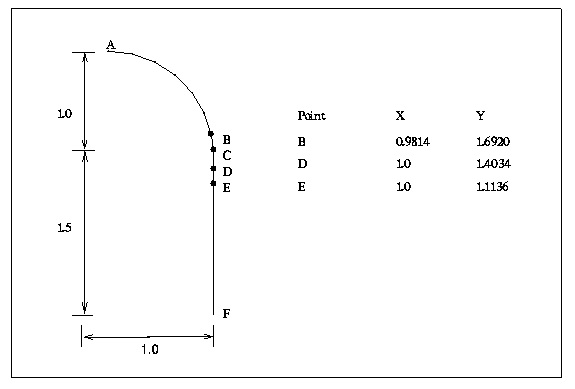
\includegraphics[width=0.7\linewidth]{./PV_1}
%\caption{}
%\label{fig:PV_1}
%\end{figure}
%
%\chapter{Belleville Washer}
%
%See Ansys Verification Problems p73.
%\begin{figure}[!h]
%\centering
%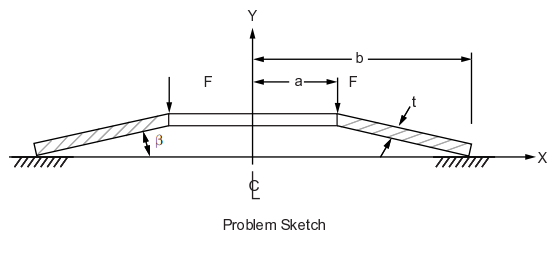
\includegraphics[width=0.7\linewidth]{./Belleville}
%\caption{}
%\label{fig:Belleville}
%\end{figure}
%
%
%\chapter{Method of manufactured solutions}
%
%\chapter{How do we construct the elements}
%we need to fix the pyfem2 element in a couple of places.
%\begin{itemize}
%\item Fix the B matrix so that we have the r term and shape function in the 3rd row of the B matrix. (Like we did in Homework 7)
%\item Fix the integrand of the K stiffness to include the r term $B^TEBrJ_\omega$
%\item Similarly fix the F term in the forcing function portion of the code.
%\end{itemize}
%
%The types of elements that we're going to focus on in this project is the reduced integration.
%
%Secondary to those, we can optionally figure out the full integration. 
%
%Listed out the order of attack for the elements we develop could be:
%\begin{itemize}
%\item Full integration (maybe easiest to implement)
%\item Reduced integration (down to one gauss point)
%\item Selectively reduced integration ????
%\item Reduced integration with hourglass control ???
%\end{itemize}
%
%The key for our project is to get the testing framework up and running for several types of loading conditions and provide something for elements to be tested against. This testing framework is the most likely thing that Fuller will re-use in pyfem2. That's most likely what he wants.
%

% % % % % % % % % % % Performance Evaluation
\chapter{Performance Evaluation}
The following section evaluates each of the elements developed (or attempted to be developed) and interrogates their performance relative to the following criteria:
\begin{itemize}
\item Convergence of a metric to a solution
\item Convergence of a metric toward the analytical solution
\item Stability of element in several loading states
\item Suitability of element under various material parameters ($E,\nu$)
\end{itemize}

As mentioned above, the primary elements of interest are the CSDAX4F (full integration) and CSDAX4R (reduced integration) elements. We attempted to develop a selective reduced integration element (CSDAX4S), however, as will be shown, the performance metrics failed so miserably, that the element is useless much more development work must take place in order for such an element to be functional. 

\section{Determining Differences Between Analytical and Numerical Solutions}
Although much more rigorous methods could likely be applied to determining the difference between the analytical and numerical solution for FEM problems, the more simple the metric, the more easily understood it is. Therefore, we determined that an acceptable metric is the maximum displacement of the plate. This maximum deflection has well defined solutions (cataloged in great detail in Roark's solution manual). 

In order to extract the maximum deflection from the FEM solution, it is critical to interrogate each node individually for its displacement in the Z axis. Therefore, the following function was constructed in order to interrogate each node for its displacement.
\begin{lstlisting}[language=Python]
def get_max_disp(V,**kwargs):
    uy_max=0
    uy_max2=0
    Xi=array(V.mesh.coord)
    ui=array(V.steps.last.dofs.reshape(Xi.shape))
    for ym in ui[:,1]:
        aym=abs(ym)
        if uy_max < aym:
            uy_max=aym
            uy_max2=ym
    return uy_max2
\end{lstlisting}

If interrogating each individual point, and comparing each FEM point to an analytical solution, a more rigorous function that returns the x \& y displacements as well as the original positions $X$ and $Y$ is:
\begin{lstlisting}[language=Python]
def get_disp_pos(GP,V,**kwargs):
    Xi=array(V.mesh.coord)
    ui=array(V.steps.last.dofs.reshape(Xi.shape))
    ux = ui[GP,0]
    uy = ui[GP,1]
    X  = Xi[GP,0]
    Y  = Xi[GP,1]
    return ux,uy,X,Y
\end{lstlisting}

Finally, if an nx4 array is desired to pass to testing functions for analysis, the following function may come in use. We did not end up implementing these functions into any of the testing framework that we developed, however, if one desired to test all points against an analytical solution, this function would be useful.
\begin{lstlisting}[language=Python]
def get_all_disp_pos(V,**kwargs):
    nnodes=V.numnod
    data = array(zeros((nnodes,4)))
    for ii in range(0,nnodes):
        data[ii,:]=get_disp_pos(ii,V)
    return data
\end{lstlisting}

\section{Convergence}
An error metric was developed which was the error between the numerical solution $Y_{num}$ and the analytical solution $Y_{a}$. Although there are many error metrics, the one determined most useful for the purposes of determining convergence upon \it{a}  solution \normalfont is a simplistic difference error. This error, which will be utilized in the vertical axis of the plots in this section and can be summarized as:
\begin{equation}
error=Y_{FEM}-Y_{a}
\end{equation}

The following listing provides a function for which one can pass an analysis system into in order to determine the errors associated with that analysis system. Note that this code also returns the number of elements and the percent error.
\begin{lstlisting}[language=Python]
def Comp_Analysis(E,v,P,OD,h,inD=None,
                  NinX=None,NinY=None,eletyp=None,formula=None,
                  Model_Comparison_Function=None,A_Mod_Comp_Fun=None,**kwargs):
    d=dict({'E':E,'v':v,'P':P,'OD':OD,'h':h,'inD':inD,'NinX':NinX,'NinY':NinY,
            'eletyp':eletyp,'formula':formula})
    V=Model_Comparison_Function(**d)
    zFEM = get_max_disp(V)
    zANA = A_Mod_Comp_Fun(**d)
    err=(zFEM-zANA)#/zANA*100.
    err2=(zFEM-zANA)/zANA*100.
    print(Model_Comparison_Function)
    print(eletyp)
    print('Numerical Sol is: ',zFEM)
    print('Analytical Sol is:',zANA)
    print('Absolute Error is:',err)
    print('Percent Error is: ',err2)
    nele=V.numele
    return err,err2,nele
\end{lstlisting}

\subsection{CSDAX4F- Full Integration}
The full integration element was the most successful in converging in nearly all loading conditions. As can be seen from the series of figures following, the element seems to follow excellent h-refinement convergence. The primary driver in this h-refinement is the generic mesh density. However, if greater detail is applied to ensuring a very square element, instead of rectangular elements, convergence is much more rapid.

In addition to this mesh dependence, it is important to note that if the mesh density in the $Z$ direction is increased without an increase in the $R$ mesh density, the model fails to converge with h-refinement. However, when both are applied (as shown in the images below), h-refinement convergence is much more rapid. 

It was generally observed that fewer than 4 elements in the $Z$ directions were unsatisfactory for producing a mesh that gave believable results for the full integration element. Not a great deal of work was exerted toward interrogating this fact, but it is notable nonetheless.


\begin{figure}[H]
\centering
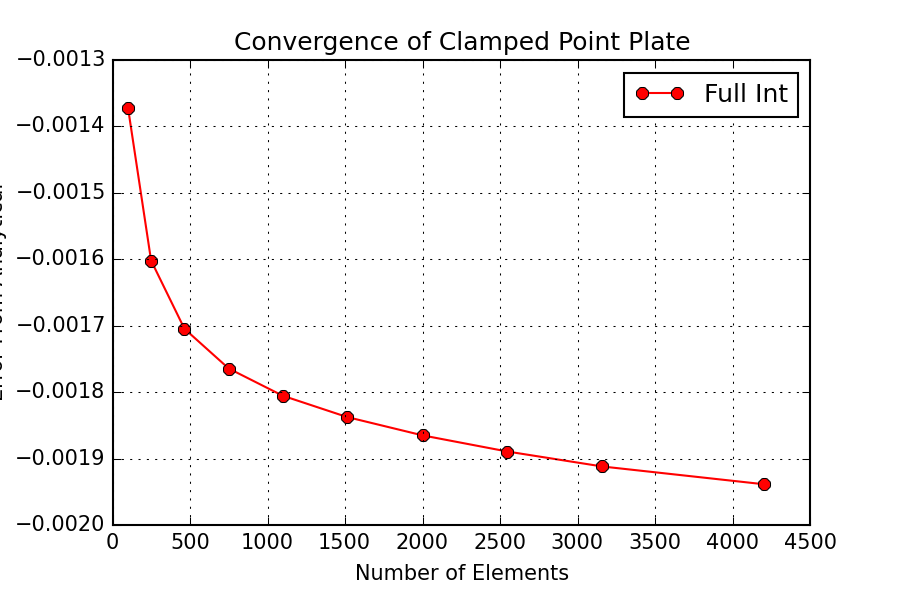
\includegraphics[width=0.7\linewidth]{./GoodImages/Conv_PlPoCl_2}
\caption[H refinement of CSDAX4F]{H refinement of CSDAX4F under the loading condition described above. This loading condition was the axisymmetric plate with a central point load and clamped outer boundary.}
\label{fig:Fig1}
\end{figure}

\begin{figure}[H]
\centering
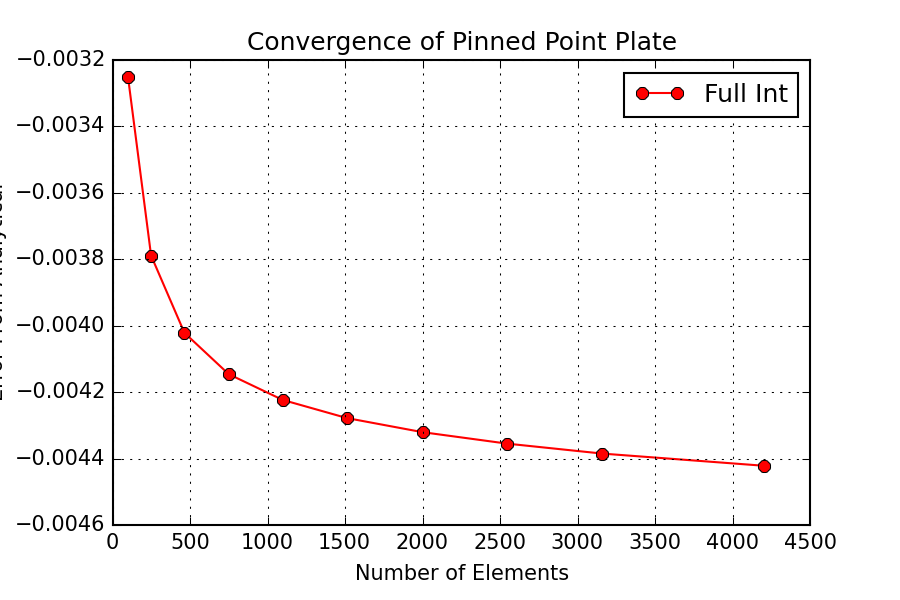
\includegraphics[width=0.7\linewidth]{./GoodImages/Conv_PlPoPi_2}
\caption[H refinement of CSDAX4F]{H refinement of CSDAX4F under the loading condition described above. This loading condition was the axisymmetric plate with a central point load and pinned outer boundary.}
\label{fig:Fig2}
\end{figure}

\begin{figure}[H]
\centering
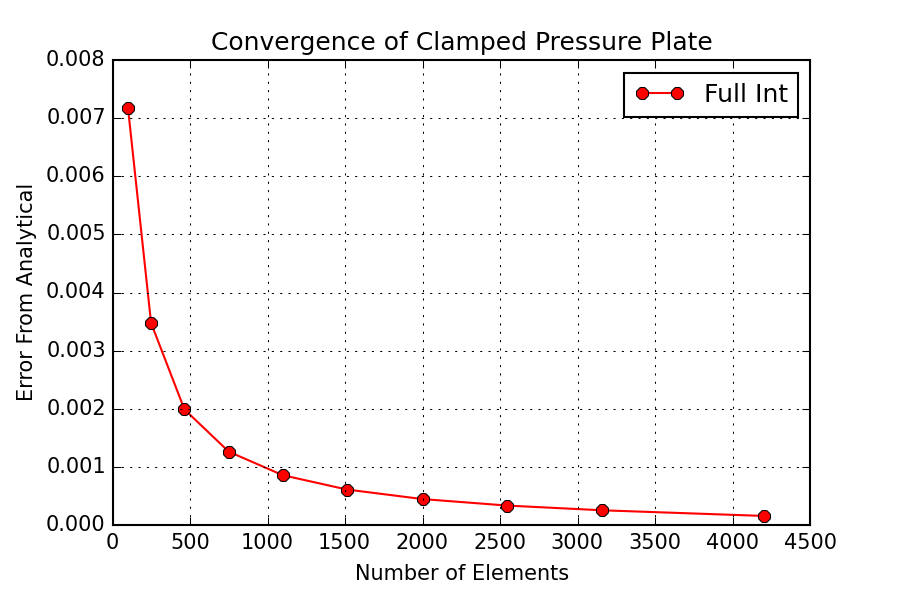
\includegraphics[width=0.7\linewidth]{./GoodImages/Conv_PlPrCl_2}
\caption[H refinement of CSDAX4F]{H refinement of CSDAX4F under the loading condition described above. This loading condition was the axisymmetric plate with a uniform pressure load and clamped outer boundary.}
\label{fig:Conv_PlPoCl_2}
\end{figure}

\begin{figure}[H]
\centering
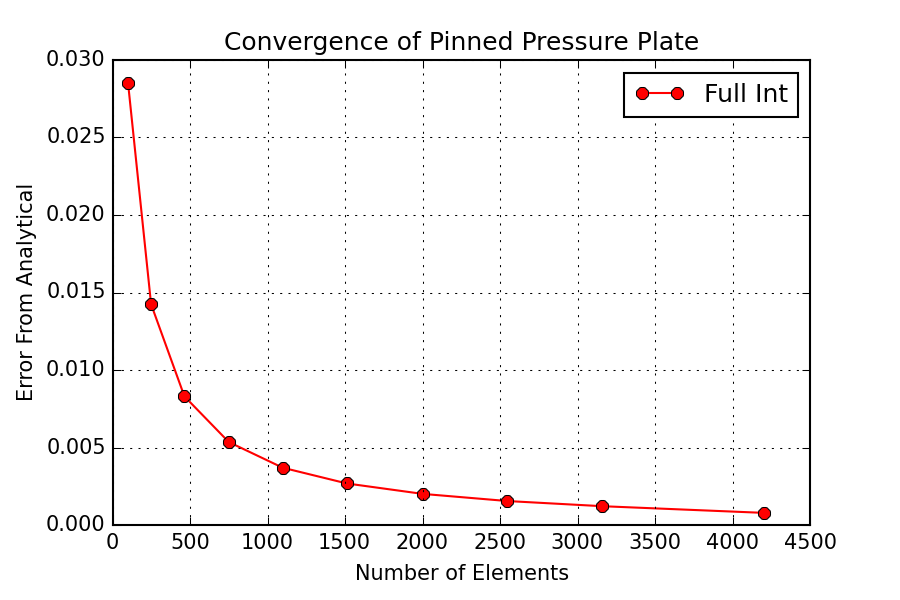
\includegraphics[width=0.7\linewidth]{./GoodImages/Conv_PlPrPi_2}
\caption[H refinement of CSDAX4F]{H refinement of CSDAX4F under the loading condition described above. This loading condition was the axisymmetric plate with a uniform pressure load and pinned outer boundary.}
\label{fig:Conv_PlPoCl_2}
\end{figure}

\begin{figure}[H]
\centering
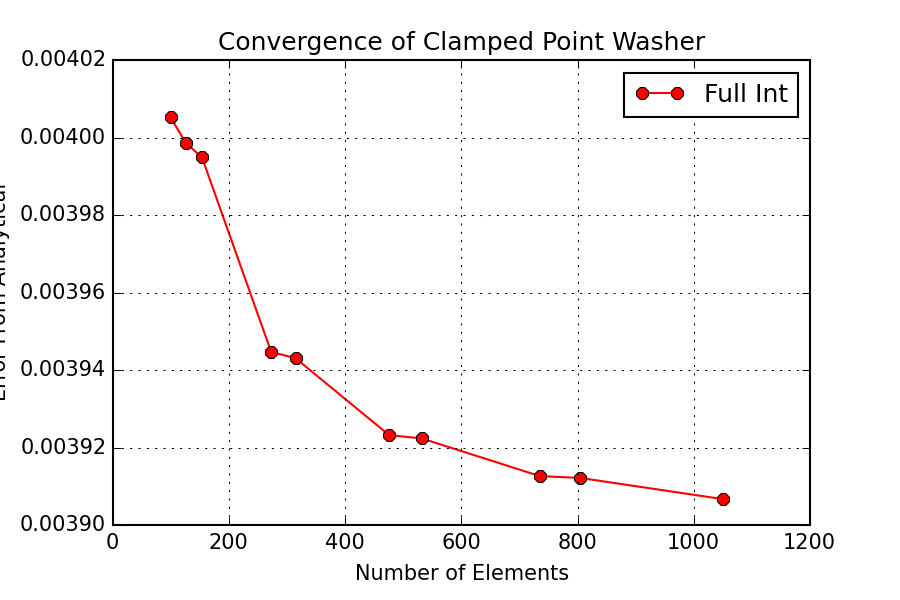
\includegraphics[width=0.7\linewidth]{./GoodImages/Conv_WaPoCl_2}
\caption[H refinement of CSDAX4F]{H refinement of CSDAX4F under the loading condition described above. This loading condition was the axisymmetric washer with a point load on the inside diameter of the washer and clamped outer boundary.}
\label{fig:Conv_PlPoCl_2}
\end{figure}

\begin{figure}[H]
\centering
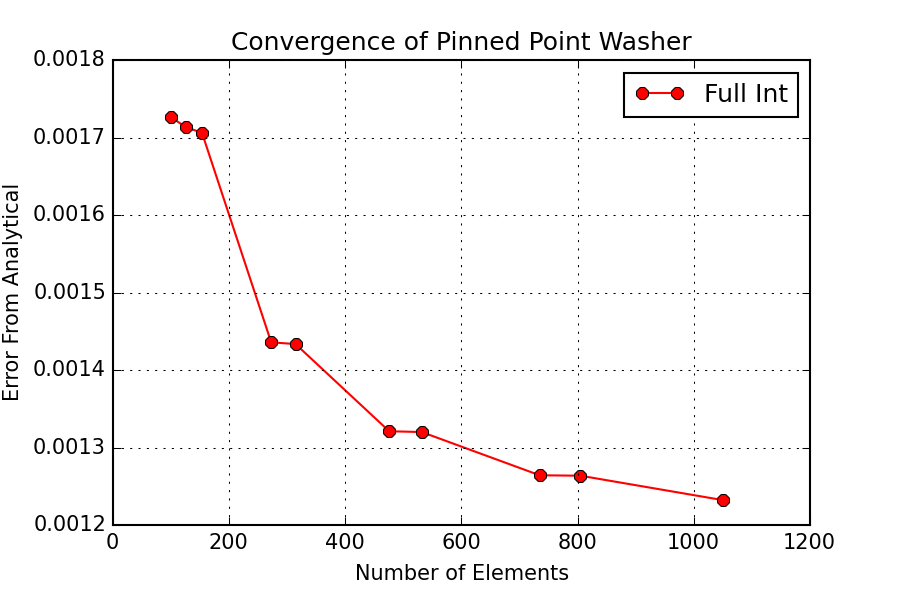
\includegraphics[width=0.7\linewidth]{./GoodImages/Conv_WaPoPi_2}
\caption[H refinement of CSDAX4F]{H refinement of CSDAX4F under the loading condition described in section ???. This loading condition was the axisymmetric washer with a point load on the inside diameter of the washer and pinned outer boundary.}
\label{fig:Conv_PlPoCl_2}
\end{figure}

\begin{figure}[H]
\centering
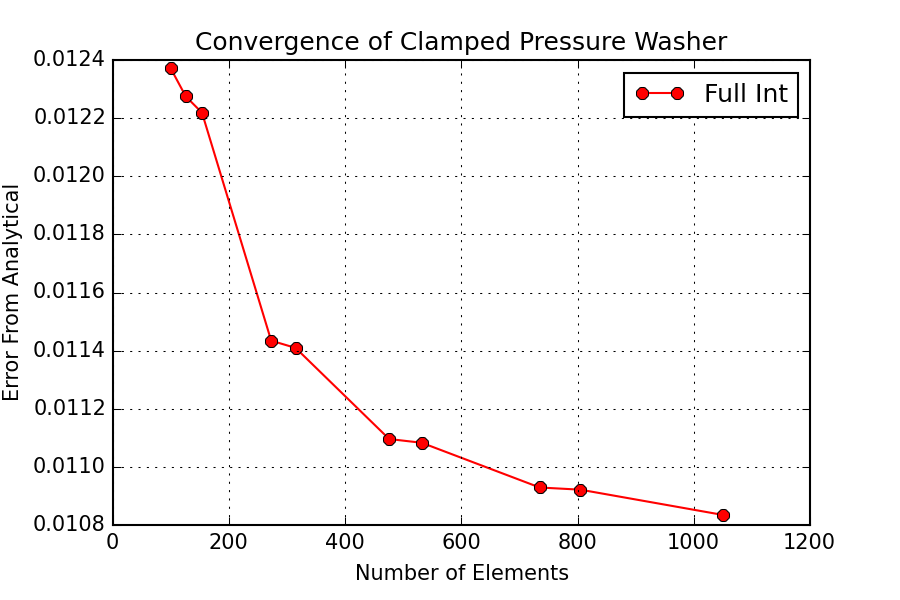
\includegraphics[width=0.7\linewidth]{./GoodImages/Conv_WaPrCl_2}
\caption[H refinement of CSDAX4F]{H refinement of CSDAX4F under the loading condition described in section ???.This loading condition was the axisymmetric washer with a uniform pressure load and clamped outer boundary.}
\label{fig:Conv_PlPoCl_2}
\end{figure}

\begin{figure}[H]
\centering
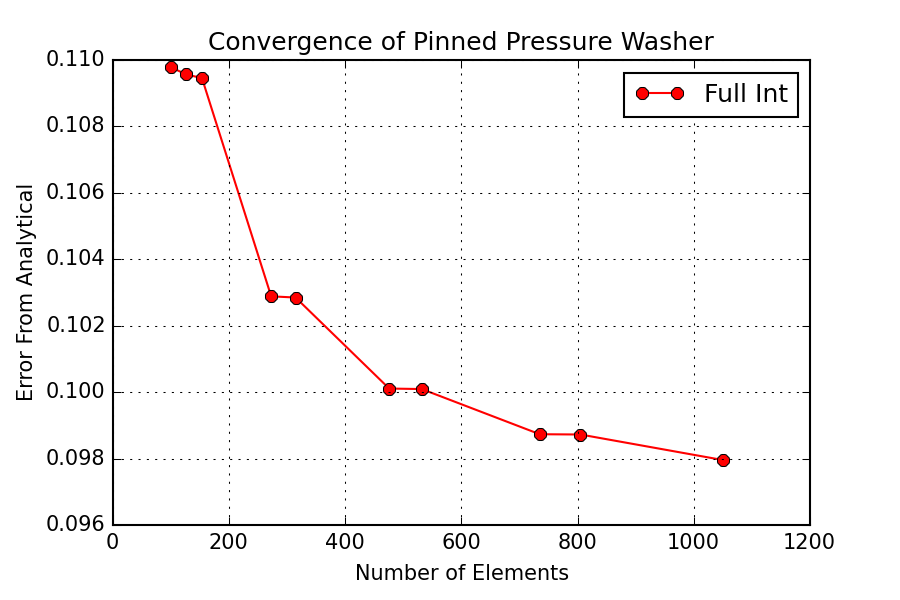
\includegraphics[width=0.7\linewidth]{./GoodImages/Conv_WaPrPi_2}
\caption[H refinement of CSDAX4F]{H refinement of CSDAX4F under the loading condition described in section ???. This loading condition was the axisymmetric washer with a uniform pressure load and pinned outer boundary.}
\label{fig:Conv_PlPoCl_2}
\end{figure}


\newpage
\subsection{CSDAX4R- Reduced Integration}
The reduced integration element struggled to converge in all loading situations. The root cause of this inconsistency is not clear, however, it is clear that whenever the pinned boundary condition is applied to the reduced integration element, the model fails to converge on a solution with h-refinement.

\begin{figure}[H]
\centering
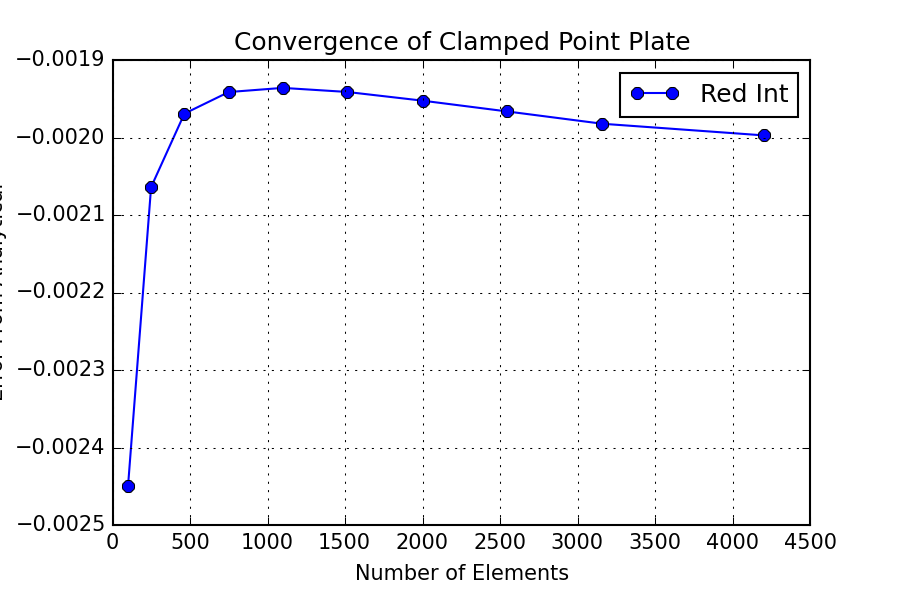
\includegraphics[width=0.7\linewidth]{./GoodImages/Conv_PlPoCl_3}
\caption[H refinement of CSDAX4R]{H refinement of CSDAX4R under the loading condition described above. This loading condition was the axisymmetric plate with a central point load and clamped outer boundary.}
\label{fig:Conv_PlPoCl_3}
\end{figure}

\begin{figure}[H]
\centering
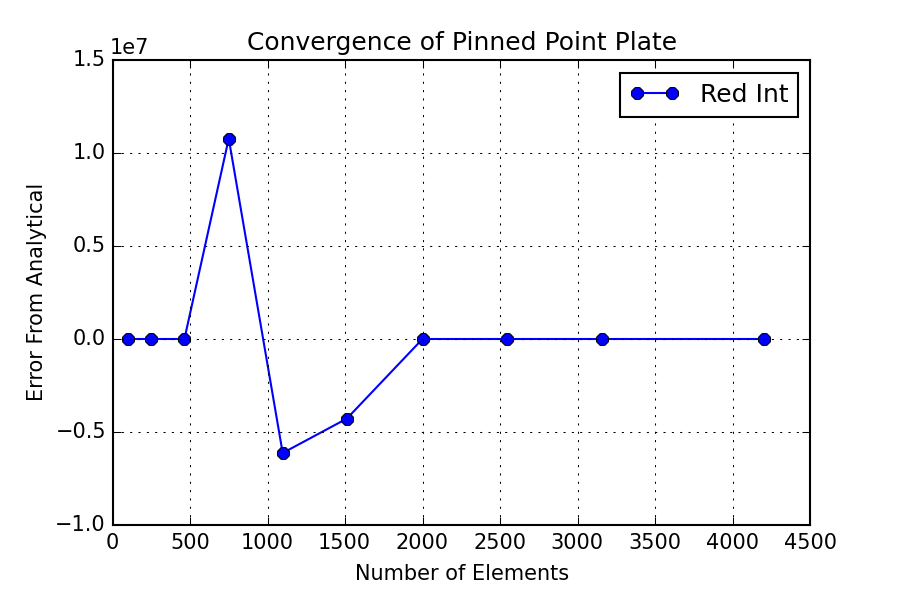
\includegraphics[width=0.7\linewidth]{./GoodImages/Conv_PlPoPi_3}
\caption[H refinement of CSDAX4R]{H refinement of CSDAX4R under the loading condition described above. This loading condition was the axisymmetric plate with a central point load and pinned outer boundary.}
\label{fig:Conv_PlPoCl_3}
\end{figure}

\begin{figure}[H]
\centering
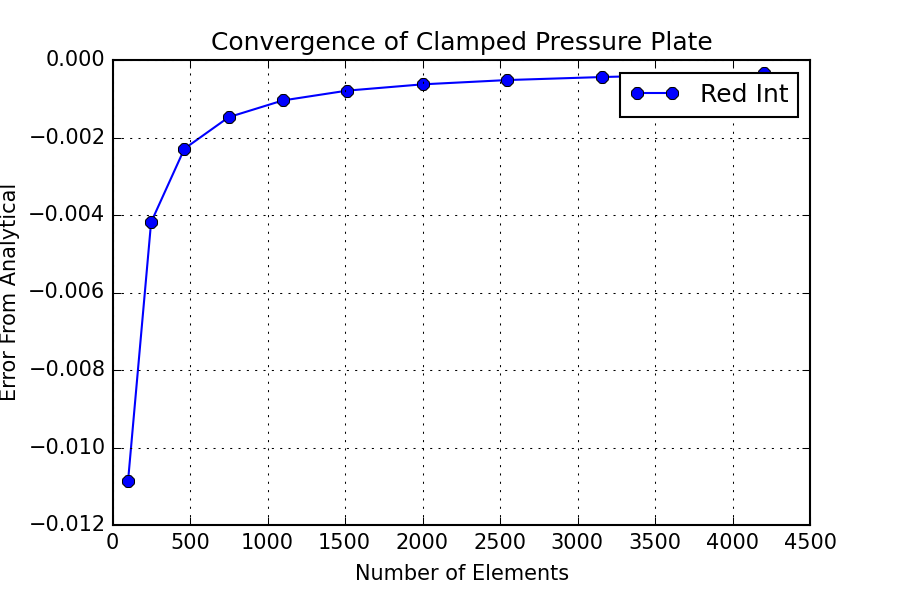
\includegraphics[width=0.7\linewidth]{./GoodImages/Conv_PlPrCl_3}
\caption[H refinement of CSDAX4R]{H refinement of CSDAX4R under the loading condition described above. This loading condition was the axisymmetric plate with a uniform pressure load and clamped outer boundary.}
\label{fig:Conv_PlPoCl_3}
\end{figure}

\begin{figure}[H]
\centering
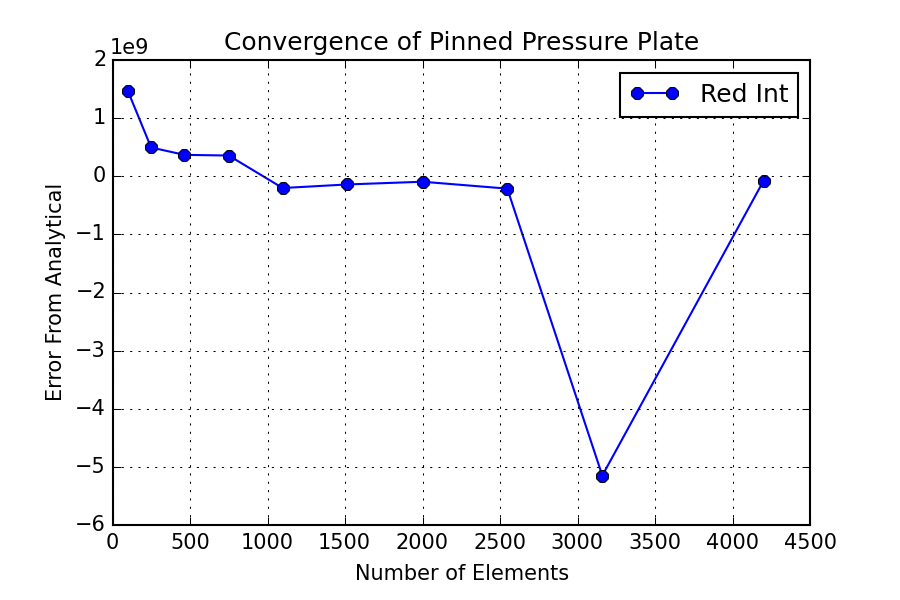
\includegraphics[width=0.7\linewidth]{./GoodImages/Conv_PlPrPi_3}
\caption[H refinement of CSDAX4R]{H refinement of CSDAX4R under the loading condition described above. This loading condition was the axisymmetric plate with a uniform pressure load and pinned outer boundary.}
\label{fig:Conv_PlPoCl_3}
\end{figure}

\begin{figure}[H]
\centering
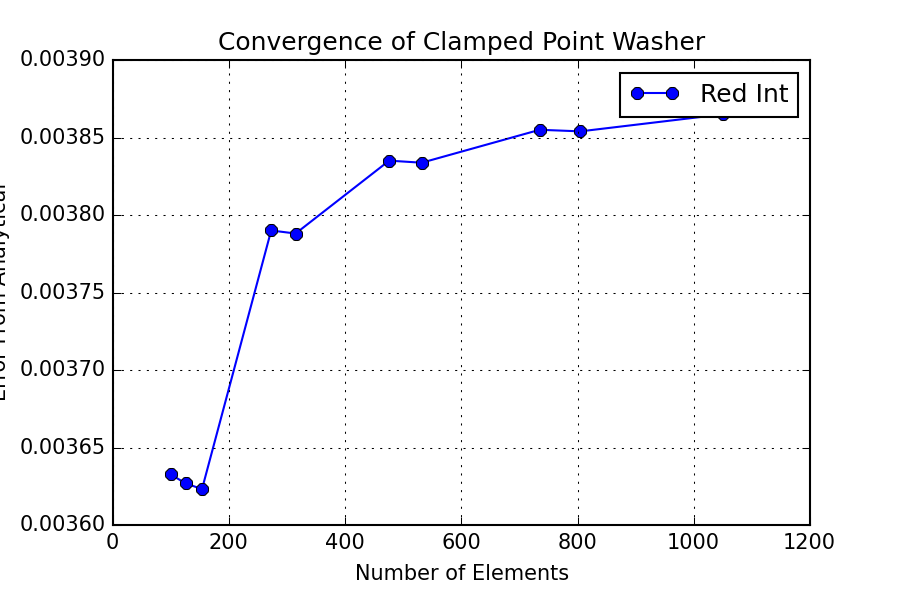
\includegraphics[width=0.7\linewidth]{./GoodImages/Conv_WaPoCl_3}
\caption[H refinement of CSDAX4R]{H refinement of CSDAX4R under the loading condition described above. This loading condition was the axisymmetric washer with a point load on the inside diameter of the washer and clamped outer boundary.}
\label{fig:Conv_PlPoCl_3}
\end{figure}

\begin{figure}[H]
\centering
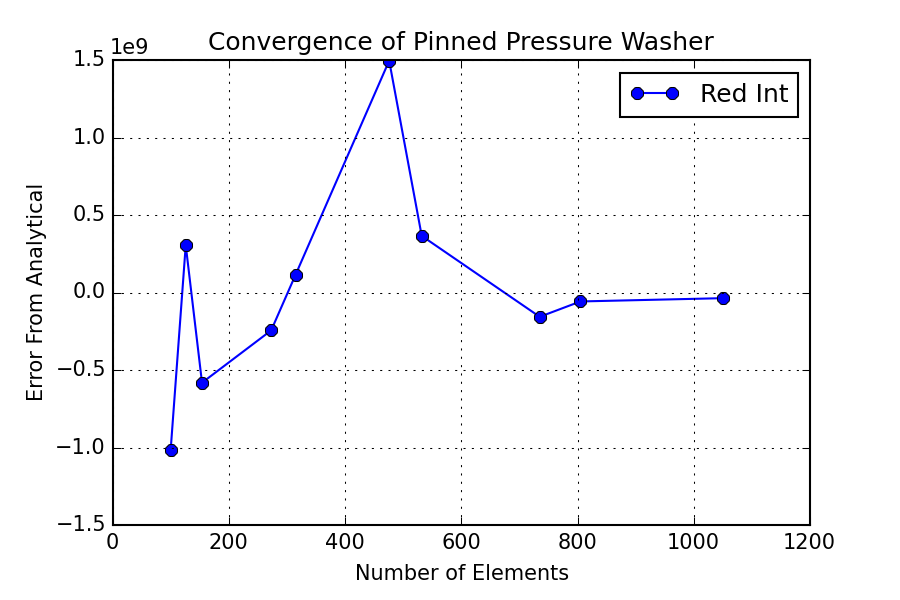
\includegraphics[width=0.7\linewidth]{./GoodImages/Conv_WaPoPi_3}
\caption[H refinement of CSDAX4R]{H refinement of CSDAX4R under the loading condition described in section ???. This loading condition was the axisymmetric washer with a point load on the inside diameter of the washer and pinned outer boundary.}
\label{fig:Conv_PlPoCl_3}
\end{figure}

\begin{figure}[H]
\centering
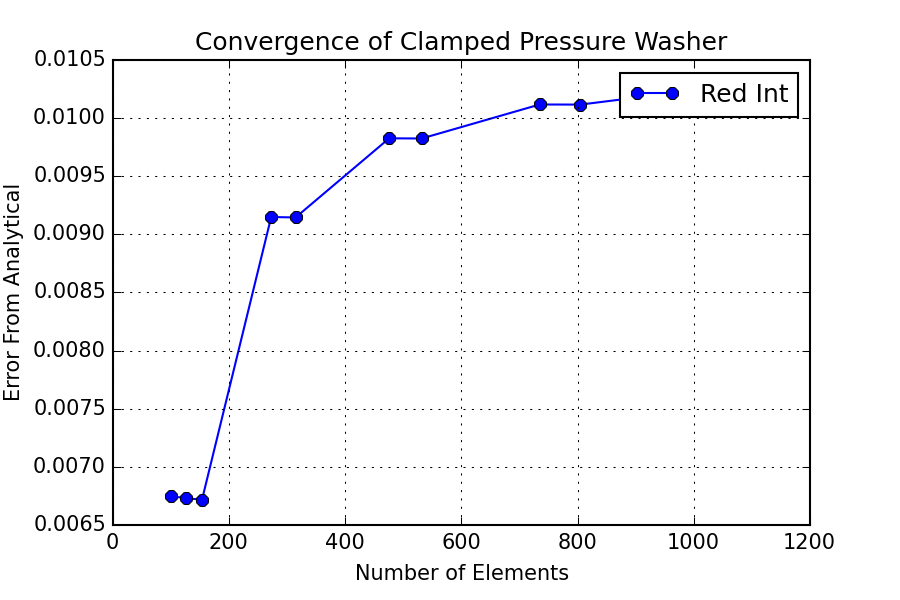
\includegraphics[width=0.7\linewidth]{./GoodImages/Conv_WaPrCl_3}
\caption[H refinement of CSDAX4R]{H refinement of CSDAX4R under the loading condition described in section ???.This loading condition was the axisymmetric washer with a uniform pressure load and clamped outer boundary.}
\label{fig:Conv_PlPoCl_3}
\end{figure}

\subsection{Comparing Convergence of Both Elements}
The following plots compare the convergence of the CSDAX4F and CSDAX4R element types. Note that some plots (particularly the plots with pinned joints) have extreme scales due to the errors and non-convergence associated with the reduced integration element. This shows that there is clearly some malfunction in the operation of the pin constraint when operating on the reduced integration eleemnt. As mentioned earlier, there is no known solution to this as of yet.

\begin{figure}[H]
\centering
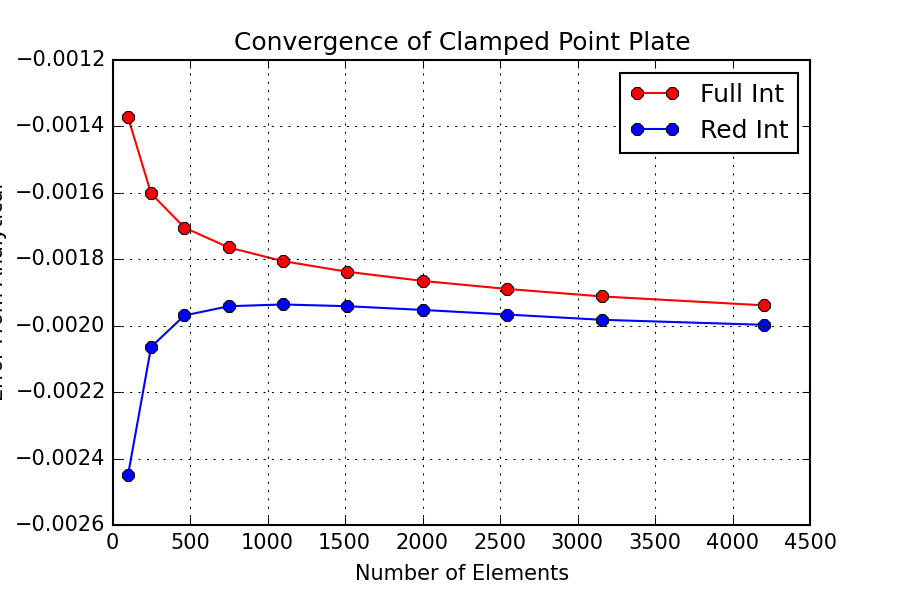
\includegraphics[width=0.7\linewidth]{./GoodImages/Conv_PlPoCl_1}
\caption[H refinement of CSDAX4F]{Comparison of CSDAX4F and CSDAX4R under the loading condition described above. This loading condition was the axisymmetric plate with a central point load and clamped outer boundary.}
\label{fig:Conv_PlPoCl_1}
\end{figure}

\begin{figure}[H]
\centering
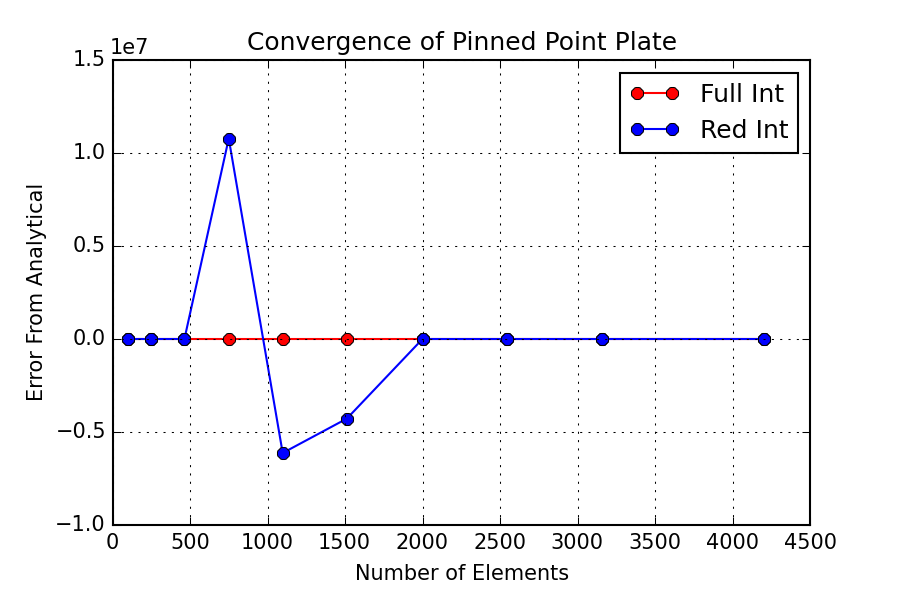
\includegraphics[width=0.7\linewidth]{./GoodImages/Conv_PlPoPi_1}
\caption[H refinement of CSDAX4F]{Comparison of CSDAX4F and CSDAX4R under the loading condition described above. This loading condition was the axisymmetric plate with a central point load and pinned outer boundary.}
\label{fig:Conv_PlPoCl_1}
\end{figure}

\begin{figure}[H]
\centering
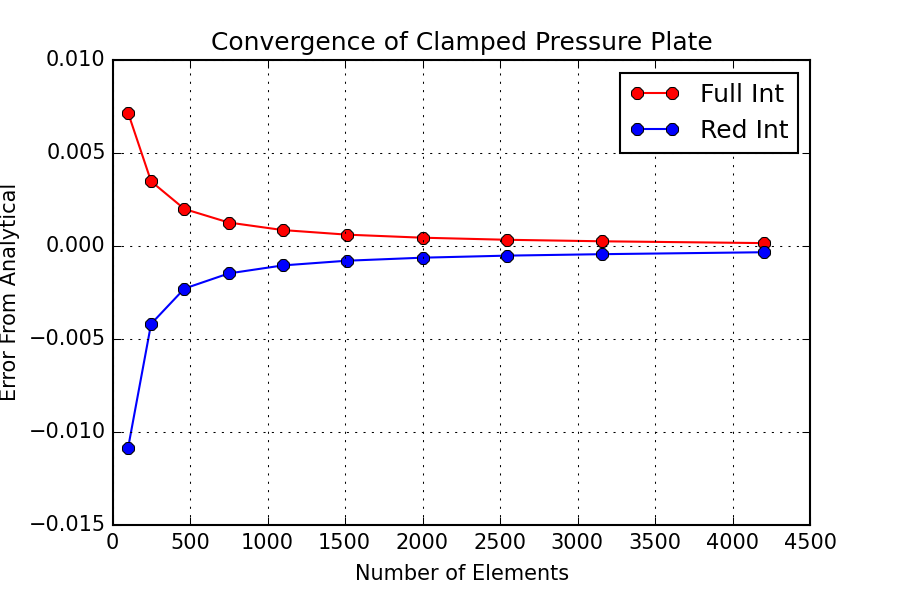
\includegraphics[width=0.7\linewidth]{./GoodImages/Conv_PlPrCl_1}
\caption[H refinement of CSDAX4F]{Comparison of CSDAX4F and CSDAX4R under the loading condition described above. This loading condition was the axisymmetric plate with a uniform pressure load and clamped outer boundary.}
\label{fig:Conv_PlPoCl_1}
\end{figure}

\begin{figure}[H]
\centering
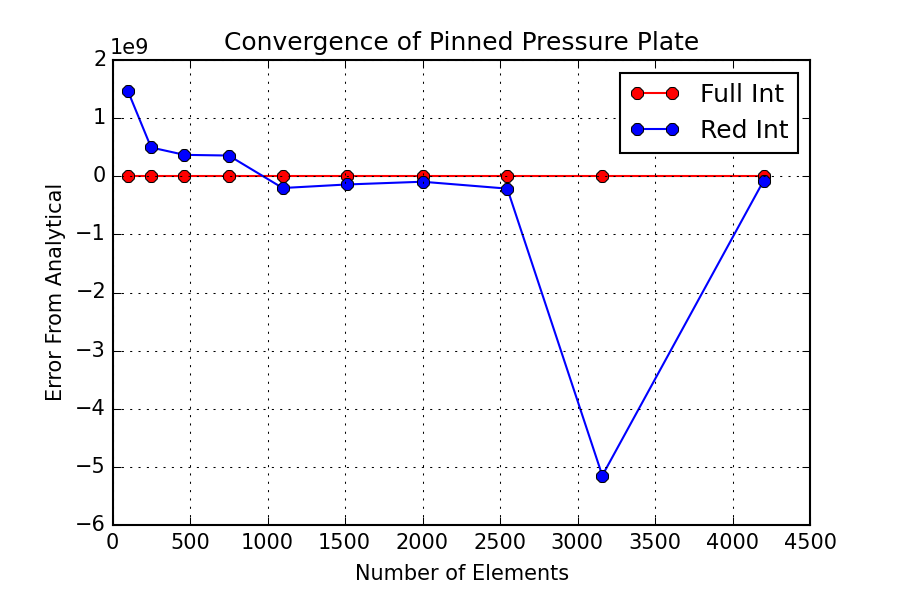
\includegraphics[width=0.7\linewidth]{./GoodImages/Conv_PlPrPi_1}
\caption[H refinement of CSDAX4F]{Comparison of CSDAX4F and CSDAX4R under the loading condition described above. This loading condition was the axisymmetric plate with a uniform pressure load and pinned outer boundary.}
\label{fig:Conv_PlPoCl_1}
\end{figure}

\begin{figure}[H]
\centering
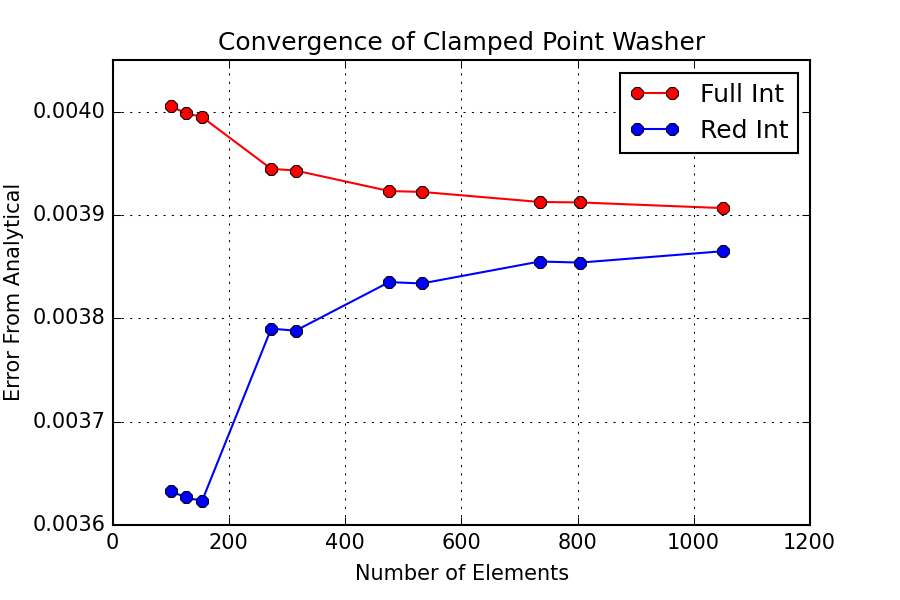
\includegraphics[width=0.7\linewidth]{./GoodImages/Conv_WaPoCl_1}
\caption[H refinement of CSDAX4F]{Comparison of CSDAX4F and CSDAX4R under the loading condition described above. This loading condition was the axisymmetric washer with a point load on the inside diameter of the washer and clamped outer boundary.}
\label{fig:Conv_PlPoCl_1}
\end{figure}

\begin{figure}[H]
\centering
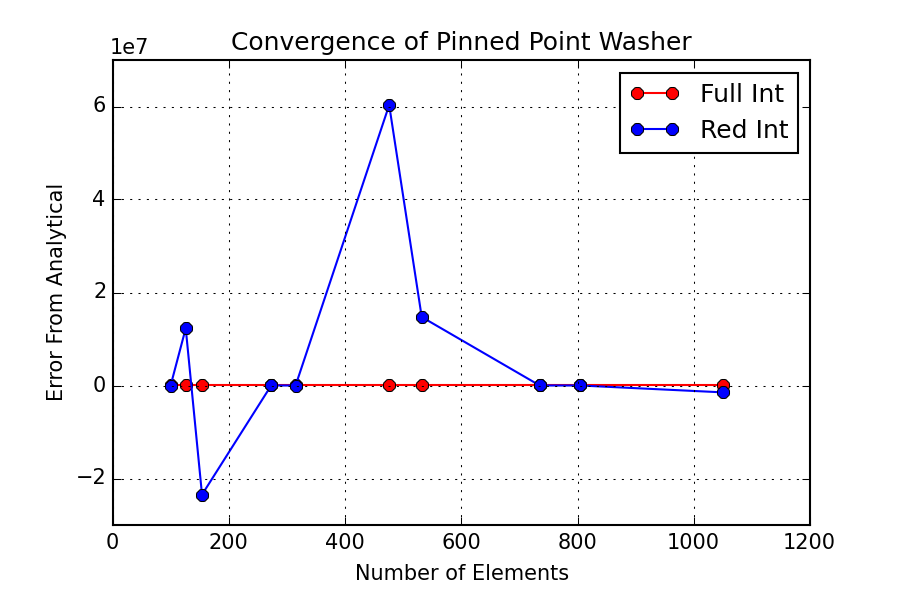
\includegraphics[width=0.7\linewidth]{./GoodImages/Conv_WaPoPi_1}
\caption[H refinement of CSDAX4F]{Comparison of CSDAX4F and CSDAX4R under the loading condition described in section ???. This loading condition was the axisymmetric washer with a point load on the inside diameter of the washer and pinned outer boundary.}
\label{fig:Conv_PlPoCl_1}
\end{figure}

\begin{figure}[H]
\centering
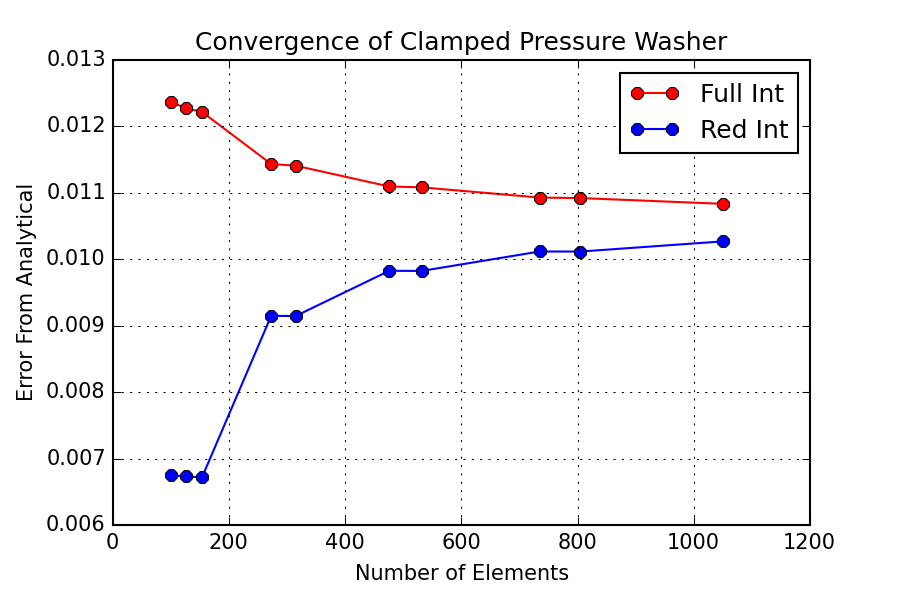
\includegraphics[width=0.7\linewidth]{./GoodImages/Conv_WaPrCl_1}
\caption[H refinement of CSDAX4F]{Comparison of CSDAX4F and CSDAX4R under the loading condition described in section ???.This loading condition was the axisymmetric washer with a uniform pressure load and clamped outer boundary.}
\label{fig:Conv_PlPoCl_1}
\end{figure}

\begin{figure}[H]
\centering
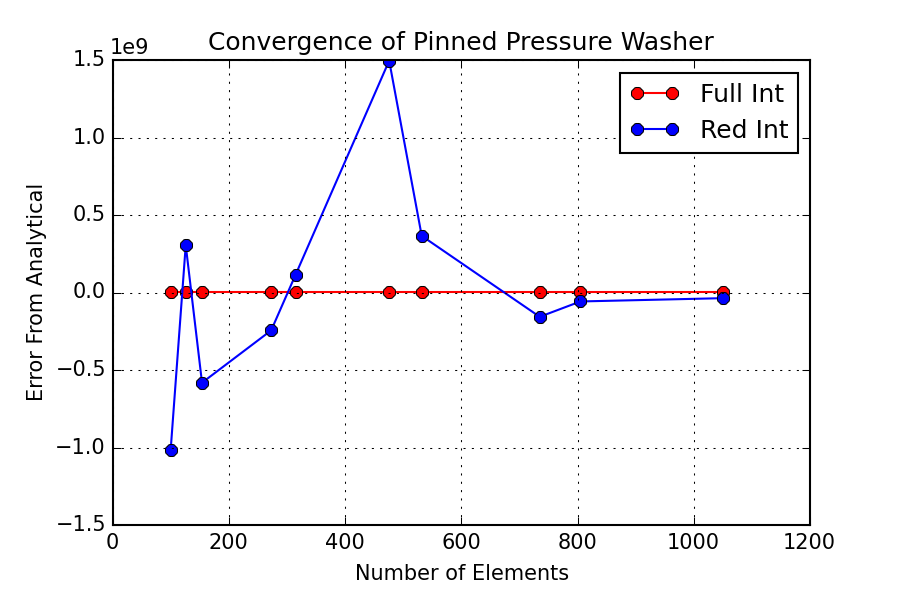
\includegraphics[width=0.7\linewidth]{./GoodImages/Conv_WaPrPi_1}
\caption[H refinement of CSDAX4F]{Comparison of CSDAX4F and CSDAX4R under the loading condition described in section ???. This loading condition was the axisymmetric washer with a uniform pressure load and pinned outer boundary.}
\label{fig:Conv_PlPoCl_1}
\end{figure}




\section{Convergence toward analytical solutions}
Convergence toward analytical solutions is somewhat sketchy at this point. This is primarily because we are unsure if the analytical solutions are providing the appropriate response to what we are observing with the finite element solutions. Because the convergence plots above do not all go to zero, this shows that there is some problems with at least a few of the analytical solutions. The analytical solutions that look very good are the clamped and pinned boundary conditions on the uniform plate (no hole) with a uniform pressure load applied. 

We are unsure, why the concentrated loads are not functioning properly, however, we suspect is has something to do with applying a concentrated load at the center of the axisymmetric element. At this point, r=0 and some rather strange things can begin to happen. Because the radius of the gauss integration point is very small, this may cause the FEM displacement to be too small. This is reflected in the h-refinement images shown in figures ~\ref{fig:Fig1} and ~\ref{fig:Fig2}. In fact, in both of those figures, the error seems to converge to a slope rather than a level.


\section{Functions utilized to determine convergence etc}
The following listings are functions that are utilized in determining the convergence of the model.
\begin{lstlisting}[language=Python]
import sys
import pdb
import matplotlib
sys.path.insert(0, '../')
from pyfem2 import *
from Definitions import *
from Definitions2 import *
from mpl_toolkits.mplot3d import Axes3D
from matplotlib import cm
from matplotlib import pyplot as plt

def find_convergence(Model_Comparison_Function,
                     A_Mod_Comp_Fun,
                     nstep=None,xmax=None,title=None,
                     saveas1=None,saveas2=None,
                     saveas3=None,saveas4=None,**kwargs):
    if nstep is None:
        nstep=7
    if xmax is None:
        xmax=200
    if title is None:
        title='Convergence on Model'
    if saveas1 is None:
        saveas1='Convergence_A.png'
    if saveas2 is None:
        saveas2='Convergence_F.png'
    if saveas2 is None:
        saveas2='Convergence_R.png'
    if saveas2 is None:
        saveas2='Convergence_S.png'
    pconv=dict({'P':40,
                'OD':23,
                'h':.4,
                'formula':1,
                'inD':23/2,
                'E':5e7,
                'v':0.4,
                'Model_Comparison_Function':Model_Comparison_Function,
                'A_Mod_Comp_Fun':A_Mod_Comp_Fun})
    ymax=int(pconv['h']*xmax/pconv['OD'])*3
    ninx=linspace(50,xmax,nstep)
    niny=linspace(3,ymax,nstep)
    
    er_f=zeros(nstep)
    ne_f=zeros(nstep)
    erp_f=zeros(nstep)
    for ii,nx in enumerate(ninx):
        pconv['NinX']=int(ninx[ii])
        pconv['NinY']=int(niny[ii])
        pconv['eletyp']=AxiSymmetricQuad4
        #er_f[ii],ne_f[ii]=Model_Comparison_Function(**pconv)
        er_f[ii],erp_f[ii],ne_f[ii]=Comp_Analysis(**pconv)
        
    er_r=zeros(nstep)
    ne_r=zeros(nstep)
    erp_r=zeros(nstep)
    for ii,nx in enumerate(ninx):
        pconv['NinX']=int(ninx[ii])
        pconv['NinY']=int(niny[ii])
        pconv['eletyp']=AxiSymmetricQuad4Reduced
        #er_r[ii],ne_r[ii]=Model_Comparison_Function(**pconv)
        er_r[ii],erp_r[ii],ne_r[ii]=Comp_Analysis(**pconv)
        
    er_s=zeros(nstep)
    ne_s=zeros(nstep)
    erp_s=zeros(nstep)
    for ii,nx in enumerate(ninx):
        pconv['NinX']=int(ninx[ii])
        pconv['NinY']=int(niny[ii])
        pconv['eletyp']=AxiSymmetricQuad4SelectiveReduced
        #er_s[ii],ne_s[ii]=Model_Comparison_Function(**pconv)
        er_s[ii],erp_s[ii],ne_s[ii]=Comp_Analysis(**pconv)
    
    plt.plot(ne_f,er_f,marker='o', linestyle='-', color='r',label='Full Int')
    plt.plot(ne_r,er_r,marker='o', linestyle='-', color='b',label='Red Int')
    #plt.plot(ne_s,er_s,marker='o', linestyle='-', color='g',label='Sel Red Int')
    plt.xlabel('Number of Elements')
    plt.ylabel('Error From Analytical')
    plt.title(title)
    plt.legend()
    plt.grid(True)
    plt.savefig(saveas1)
    plt.show()
    
    
    plt.plot(ne_f,er_f,marker='o', linestyle='-', color='r',label='Full Int')
    #plt.plot(ne_r,er_r,marker='o', linestyle='-', color='b',label='Red Int')
    #plt.plot(ne_s,er_s,marker='o', linestyle='-', color='g',label='Sel Red Int')
    plt.xlabel('Number of Elements')
    plt.ylabel('Error From Analytical')
    plt.title(title)
    plt.legend()
    plt.grid(True)
    plt.savefig(saveas2)    
    plt.show()
    
    #plt.plot(ne_f,er_f,marker='o', linestyle='-', color='r',label='Full Int')
    plt.plot(ne_r,er_r,marker='o', linestyle='-', color='b',label='Red Int')
    #plt.plot(ne_s,er_s,marker='o', linestyle='-', color='g',label='Sel Red Int')
    plt.xlabel('Number of Elements')
    plt.ylabel('Error From Analytical')
    plt.title(title)
    plt.legend()
    plt.grid(True)
    plt.savefig(saveas3)    
    plt.show()
    
    #plt.plot(ne_f,er_f,marker='o', linestyle='-', color='r',label='Full Int')
    #plt.plot(ne_r,er_r,marker='o', linestyle='-', color='b',label='Red Int')
    plt.plot(ne_s,er_s,marker='o', linestyle='-', color='g',label='Sel Red Int')
    plt.xlabel('Number of Elements')
    plt.ylabel('Error From Analytical')
    plt.title(title)
    plt.legend()
    plt.grid(True)
    plt.savefig(saveas4)    
    plt.show()
\end{lstlisting}

The following listing describes one potential dictionary and function call of the above definition:
\begin{lstlisting}[language=Python]
pdict=dict({'Model_Comparison_Function':Plate_Point_Pinned,
            'A_Mod_Comp_Fun':A_Plate_Point_Pinned,
            'nstep':nsteps,
            'xmax': 350,
            'title':'Convergence of Pinned Point Plate',
            'saveas1':'Conv_PlPoPi_1.png',
            'saveas2':'Conv_PlPoPi_2.png',
            'saveas3':'Conv_PlPoPi_3.png',
            'saveas4':'Conv_PlPoPi_4.png'})
find_convergence(**pdict)
\end{lstlisting}
\section{FEM code}
The following listing provides functions for each of the analysis systems described above. The naming convention is quite plain. Several FEM function definitions were not utilized in this report, however, they are given for future reference. One notable function is the thick walled pressure vessel function.

\begin{lstlisting}[language=Python]
def Plate_Point_Pinned(E,v,P,OD,h,
                       NinX=None,NinY=None,eletyp=None,formula=None,
                       **kwargs):
    if eletyp is None:
        eletyp = AxiSymmetricQuad4
    if NinX is None:
        NinX = 100 #Number of elements in I (Diameter)
    if NinY is None:
        NinY = 4 #Number elements in J (Thickness)
    if formula is None:
        formula=1
    R=OD/2.0
    kp1=NinY*(NinX+1)+1 #Central point
    kp2=NinX+1         #Bottom outside edge
    mesh = RectilinearMesh2D(nx=NinX, ny=NinY, lx=R, ly=h)
    mat = Material('Material-1', elastic={'E':E, 'Nu':v})
    
    V = FiniteElementModel(mesh=mesh, jobid='PlatePointPinned')
    V.ElementBlock('ElementBlock1', ALL)
    V.AssignProperties('ElementBlock1', eletyp, mat, formulation=formula)
    
    #V.PrescribedBC(kp2,Y)
    step = V.StaticStep()
    step.PinNodes(kp2)
    #step.FixNodes(kp2)
    #step.PrescribedBC(kp2,Y)
    step = V.StaticStep()
    step.ConcentratedLoad(kp1, Y, -P)
    step.run()
    V.WriteResults()
    if not os.environ.get('NOGRAPHICS'):
        V.Plot2D(show=1, deformed=1)
    return V

def Plate_Point_Clamped(E,v,P,OD,h,
                        NinX=None,NinY=None,eletyp=None,formula=None,
                        **kwargs):
    if eletyp is None:
        eletyp = AxiSymmetricQuad4
    if NinX is None:
        NinX=100 #Number of elements in I (Diameter)
    if NinY is None:
        NinY=4 #Number elements in J (Thickness)
    if formula is None:
        formula=1
    R=OD/2.0
    #Find Keypoints of interest
    kp1=NinY*(NinX+1)+1 #Central point
    kp2=NinX+1         #Bottom outside edge
    
    mesh = RectilinearMesh2D(nx=NinX, ny=NinY, lx=R, ly=h)
    mat = Material('Material-1', elastic={'E':E, 'Nu':v})
    
    V = FiniteElementModel(mesh=mesh, jobid='PlatePointClamped')
    V.ElementBlock('ElementBlock1', ALL)
    V.AssignProperties('ElementBlock1', eletyp, mat, formulation=formula)
    
    step = V.StaticStep()
    step.FixNodes(IHI)
    step = V.StaticStep()
    step.ConcentratedLoad(kp1, Y, -P)
    step.run()
    V.WriteResults()
    if not os.environ.get('NOGRAPHICS'):
        V.Plot2D(show=1, deformed=1)
    return V

def Plate_Pressure_Pinned(E,v,P,OD,h,
                          NinX=None,NinY=None,eletyp=None,formula=None,
                          **kwargs):
    if eletyp is None:
        eletyp = AxiSymmetricQuad4
    if NinX is None:
        NinX = 100 #Number of elements in I (Diameter)
    if NinY is None:
        NinY = 4 #Number elements in J (Thickness)
    if formula is None:
        formula=1
    R=OD/2.0
    kp1=NinY*(NinX+1)+1 #Central point
    kp2=NinX+1         #Bottom outside edge
    mesh = RectilinearMesh2D(nx=NinX, ny=NinY, lx=R, ly=h)
    mat = Material('Material-1', elastic={'E':E, 'Nu':v})
    
    V = FiniteElementModel(mesh=mesh, jobid='PlatePressurePinned')
    V.ElementBlock('ElementBlock1', ALL)
    V.AssignProperties('ElementBlock1', eletyp, mat, formulation=formula)
    
    #V.PrescribedBC(kp2,Y)
    step = V.StaticStep()
    step.PinNodes(kp2)
    #step.FixNodes(kp2)
    #step.PrescribedBC(kp2,Y)
    step = V.StaticStep()
    step.Pressure(JHI, P)
    step.run()
    V.WriteResults()
    if not os.environ.get('NOGRAPHICS'):
        V.Plot2D(show=1, deformed=1)
    return V


def Plate_Pressure_Clamped(E,v,P,OD,h,
                           NinX=None,NinY=None,eletyp=None,formula=None,
                           **kwargs):
    if eletyp is None:
        eletyp = AxiSymmetricQuad4
    if NinX is None:
        NinX = 100 #Number of elements in I (Diameter)
    if NinY is None:
        NinY = 4 #Number elements in J (Thickness)
    if formula is None:
        formula=1    
    R=OD/2.0
    kp1=NinY*(NinX+1)+1 #Central point
    kp2=NinX+1         #Bottom outside edge
    mesh = RectilinearMesh2D(nx=NinX, ny=NinY, lx=R, ly=h)
    mat = Material('Material-1', elastic={'E':E, 'Nu':v})
    
    V = FiniteElementModel(mesh=mesh, jobid='PlatePointPinned')
    V.ElementBlock('ElementBlock1', ALL)
    V.AssignProperties('ElementBlock1', eletyp, mat)
    
    step = V.StaticStep()
    step.FixNodes(IHI)
    step = V.StaticStep()
    step.Pressure(JHI, P)
    step.run()
    V.WriteResults()
    if not os.environ.get('NOGRAPHICS'):
        V.Plot2D(show=1, deformed=1)
    return V

def Washer_Point_Pinned(E,v,P,OD,h,
                        NinX=None,NinY=None,eletyp=None,inD=None,formula=None,
                        **kwargs):
    if eletyp is None:
        eletyp = AxiSymmetricQuad4
    if NinX is None:
        NinX = 50 #Number of elements in I (Diameter)
    if NinY is None:
        NinY = 4 #Number elements in J (Thickness)
    if inD is None:
        inD = OD/2.0 
    if formula is None:
        formula=1
    R  = OD/2.0
    Ri = inD/2.0
    w  = R-Ri
    kp1=NinY*(NinX+1)+1 #Central point
    kp2=NinX+1         #Bottom outside edge
    mesh = RectilinearMesh2D(nx=NinX, ny=NinY, lx=w, ly=h,shift=[Ri,0])
    mat = Material('Material-1', elastic={'E':E, 'Nu':v})
    
    V = FiniteElementModel(mesh=mesh, jobid='WasherPointPinned')
    V.ElementBlock('ElementBlock1', ALL)
    V.AssignProperties('ElementBlock1', eletyp, mat)
    
    #V.PrescribedBC(kp2,Y)
    step = V.StaticStep()
    step.PinNodes(kp2)
    #step.FixNodes(kp2)
    #step.PrescribedBC(kp2,Y)
    step = V.StaticStep()
    step.ConcentratedLoad(kp1, Y, -P)
    step.run()
    V.WriteResults()
    if not os.environ.get('NOGRAPHICS'):
        V.Plot2D(show=1, deformed=1)
    return V

def Washer_Point_Clamped(E,v,P,OD,h,
                         NinX=None,NinY=None,eletyp=None,inD=None,formula=None,
                         **kwargs):
    if eletyp is None:
        eletyp = AxiSymmetricQuad4
    if NinX is None:
        NinX = 50 #Number of elements in I (Diameter)
    if NinY is None:
        NinY = 4 #Number elements in J (Thickness)
    if inD is None:
        inD = OD/2.0 
    if formula is None:
        formula=1
    R  = OD/2.0
    Ri = inD/2.0
    w  = R-Ri
    kp1=NinY*(NinX+1)+1 #Central point
    kp2=NinX+1         #Bottom outside edge
    mesh = RectilinearMesh2D(nx=NinX, ny=NinY, lx=w, ly=h,shift=[Ri,0])
    mat = Material('Material-1', elastic={'E':E, 'Nu':v})
    
    V = FiniteElementModel(mesh=mesh, jobid='WasherPointClamped')
    V.ElementBlock('ElementBlock1', ALL)
    V.AssignProperties('ElementBlock1', eletyp, mat)
    
    step = V.StaticStep()
    step.FixNodes(IHI)
    step = V.StaticStep()
    step.ConcentratedLoad(kp1, Y, -P)
    step.run()
    V.WriteResults()
    if not os.environ.get('NOGRAPHICS'):
        V.Plot2D(show=1, deformed=1)
    return V

def Washer_Pressure_Pinned(E,v,P,OD,h,
                           NinX=None,NinY=None,eletyp=None,inD=None,formula=None,
                           **kwargs):
    if eletyp is None:
        eletyp = AxiSymmetricQuad4
    if NinX is None:
        NinX = 50 #Number of elements in I (Diameter)
    if NinY is None:
        NinY = 4 #Number elements in J (Thickness)
    if inD is None:
        inD = OD/2.0 
    if formula is None:
        formula=1
    R  = OD/2.0
    Ri = inD/2.0
    w  = R-Ri
    kp1=NinY*(NinX+1)+1 #Central point
    kp2=NinX+1         #Bottom outside edge
    mesh = RectilinearMesh2D(nx=NinX, ny=NinY, lx=w, ly=h,shift=[Ri,0])
    mat = Material('Material-1', elastic={'E':E, 'Nu':v})
    
    V = FiniteElementModel(mesh=mesh, jobid='WasherPressurePinned')
    V.ElementBlock('ElementBlock1', ALL)
    V.AssignProperties('ElementBlock1', eletyp, mat)
    
    #V.PrescribedBC(kp2,Y)
    step = V.StaticStep()
    step.PinNodes(kp2)
    #step.FixNodes(kp2)
    #step.PrescribedBC(kp2,Y)
    step = V.StaticStep()
    step.Pressure(JHI, P)
    step.run()
    V.WriteResults()
    if not os.environ.get('NOGRAPHICS'):
        V.Plot2D(show=1, deformed=1)
    return V

def Washer_Pressure_Clamped(E,v,P,OD,h,
                            NinX=None,NinY=None,eletyp=None,inD=None,formula=None,
                            **kwargs):
    if eletyp is None:
        eletyp = AxiSymmetricQuad4
    if NinX is None:
        NinX = 50 #Number of elements in I (Diameter)
    if NinY is None:
        NinY = 4 #Number elements in J (Thickness)
    if inD is None:
        inD = OD/2.0 
    if formula is None:
        formula=1
    R  = OD/2.0
    Ri = inD/2.0
    w  = R-Ri
    kp1=NinY*(NinX+1)+1 #Central point
    kp2=NinX+1         #Bottom outside edge
    mesh = RectilinearMesh2D(nx=NinX, ny=NinY, lx=w, ly=h,shift=[Ri,0])
    mat = Material('Material-1', elastic={'E':E, 'Nu':v})
    
    V = FiniteElementModel(mesh=mesh, jobid='WasherPressurePinned')
    V.ElementBlock('ElementBlock1', ALL)
    V.AssignProperties('ElementBlock1', eletyp, mat)
    
    step = V.StaticStep()
    step.FixNodes(IHI)
    step = V.StaticStep()
    step.Pressure(JHI, P)
    step.run()
    V.WriteResults()
    if not os.environ.get('NOGRAPHICS'):
        V.Plot2D(show=1, deformed=1)
    return V
    
def Universal_Plate(E,v,P,OD,h,Plate=None,Pin=None,Point=None,
                            NinX=None,NinY=None,eletyp=None,inD=None,
                            formula=None,job=None,**kwargs):
    if eletyp is None:
        eletyp = AxiSymmetricQuad4
    if NinX is None:
        NinX = 50 #Number of elements in I (Diameter)
    if NinY is None:
        NinY = 4 #Number elements in J (Thickness)
    if inD is None:
        inD = OD/2.0 
    if formula is None:
        formula=1
    if Plate is None:
        Plate = True
    if Pin is None:
        Pin = True
    if Point is None:
        Point = True
    if job is None:
        job = 'AxiSymPlate'
    R  = OD/2.0
    Ri = inD/2.0
    w  = R-Ri
    kp1=NinY*(NinX+1)+1 #Central point
    kp2=NinX+1         #Bottom outside edge
    mat = Material('Material-1', elastic={'E':E, 'Nu':v})
    
    #Case Structure for Plate vs Washer
    if Plate:
        #If Plate        
        mesh = RectilinearMesh2D(nx=NinX, ny=NinY, lx=R, ly=h)
    else:
        #If Washer
        mesh = RectilinearMesh2D(nx=NinX, ny=NinY, lx=w, ly=h,shift=[Ri,0])
    
    V = FiniteElementModel(mesh=mesh, jobid=job)
    V.ElementBlock('ElementBlock1', ALL)
    V.AssignProperties('ElementBlock1', eletyp, mat)
    step = V.StaticStep()
    # Case Structure for Pined vs Fixed Outside Diameter
    if Pin:
        step.PrescribedBC(kp2,Y)
    else:
        step.FixNodes(IHI)
    
    step = V.StaticStep()
    # Case Structure for Pressure vs Point loading
    if Point:
        step.ConcentratedLoad(kp1, Y, -P)
    else:
        step.Pressure(JHI, P)
    
    step.run()
    #V.WriteResults()
    if not os.environ.get('NOGRAPHICS'):
        V.Plot2D(show=1, deformed=1)
    return V


def Thick_Infinite_Cyl(E,v,P,OD,h,
                       NinX=None,NinY=None,eletyp=None,inD=None,formula=None,
                       **kwargs):
    if eletyp is None:
        eletyp = AxiSymmetricQuad4
    if NinX is None:
        NinX = 60 #Number of elements in I (Diameter)
    if NinY is None:
        NinY = 10 #Number elements in J (Thickness)
    if inD is None:
        inD = OD/2.0 
    if formula is None:
        formula=1
    R  = OD/2.0
    Ri = inD/2.0
    w  = R-Ri
    kp1=NinY*(NinX+1)+1 #Central point
    kp2=NinX+1         #Bottom outside edge
    mesh = RectilinearMesh2D(nx=NinX, ny=NinY, lx=w, ly=h,shift=[Ri,0])
    mat = Material('Material-1', elastic={'E':E, 'Nu':v})
    
    V = FiniteElementModel(mesh=mesh, jobid='InfiniteCylinder')
    V.ElementBlock('ElementBlock1', ALL)
    V.AssignProperties('ElementBlock1', eletyp, mat)
    
    
    V.PrescribedBC(JLO,Y)
    V.PrescribedBC(JHI,Y)
    
    #step = V.StaticStep()
    #step.FixNodes(IHI)
    step = V.StaticStep()
    step.Pressure(ILO, P)
    step.run()
    V.WriteResults()
    if not os.environ.get('NOGRAPHICS'):
        V.Plot2D(show=1, deformed=1)
    return V
\end{lstlisting}


\chapter{Unit Testing}
In general, due to non-convergence poor fitting with the analytical solutions that we were unable to resolve, unit testing was not completed. However, many of the commented assertion statements could be uncommented if the analytical solutions and the numerical solutions were in the same ballpark. If run as is, all tests would fail. 

Many more tests were planned, including tests of various poisson ratio, young's modulus, element type etc for each of the 8 loading conditions studied in this paper. The primary framework exists, however, is ultimately unsuccessful at this point.

\begin{lstlisting}
import os
import numpy as np
import subprocess
import sys
import pdb
sys.path.insert(0, '../')
from pyfem2 import *
from Definitions import *
from Definitions2 import *

#This code utilizes the testing framework within python to run verification tests on the FEM solver that we have developed.

def test_1():
    # TEST CASE 1
    # Geometry: Flat circular plate with no holes
    # Supports: Simply supported at radius r
    # Loads:    Uniform pressure load across entire plate
    # ELEMENT TYPE: AxiSymmetricQuad4
    #
    # Objective of test: 
    # Verify that element in development produces appropriate maximum 
    # deflection at the center of the plate. 
    # See schematic in documentation for more information.
    
    #### Problem Setup ####
    problem = dict({'E':1e6,
                    'v':0.3,
                    'P': 10,
                    'OD':23,
                    'h' : .4,
                    'eletyp':AxiSymmetricQuad4,
                    'formula':1})
    
    ####-----FEM-----####
    V=Plate_Pressure_Pinned(**problem)
    zFEM=get_max_disp(V)
    ####-----Exact-----####
    zANA=A_Plate_Pressure_Pinned(**problem)
    
    print(zFEM)
    print(zANA)
    err=(zFEM-zANA)/zANA*100.
    print(err)
    #Compare the solutions
    #Assert a tolerable error to pass/fail test
    #assert np.allclose(zFEM,zANA,atol=1e-5)

def test_2():
    # TEST CASE 2
    # Geometry: Flat circular plate with no holes
    # Supports: Cantilever or clamped edges at radius r
    # Loads: 	Uniform pressure load across entire plate
    #
    # Objective of test: 
    # Verify that element in development produces appropriate maximum deflection at the center of the plate. 
    # See schematic in documentation (XXXX) for more information.
    
    #### Problem Setup ####
    problem = dict({'E':1e6,
                    'v':0.3,
                    'P': 10,
                    'OD':23,
                    'h' : .4,
                    'eletyp':AxiSymmetricQuad4,
                    'formula':1})
    
    ####-----FEM-----####
    V=Plate_Pressure_Clamped(**problem)
    zFEM=get_max_disp(V)
    ####-----Exact-----####
    zANA=-A_Plate_Pressure_Clamped(**problem)
    
    print(zFEM)
    print(zANA)
    
    err=(zFEM-zANA)/zANA*100.
    print(err)
    #Compare the solutions
    #Assert a tolerable error to pass/fail test
    #assert np.allclose(zFEM,zmax,atol=1e-10)

def test_3():
    # TEST CASE 3: Plate Point Pinned
    # Geometry: Flat circular plate with no holes
    # Supports: Simply supported at Ds
    # Loads: 	Force per circumference applied at Dl
    #
    # Objective of test: 
    # Verify that element in development produces appropriate maximum deflection at the center of the plate. 
    # See schematic in documentation (XXXX) for more information.
    
    #### Problem Setup ####
    problem = dict({'E':1e6,
                    'v':0.3,
                    'P': 100,
                    'OD':23,
                    'h' : .4,
                    'eletyp':AxiSymmetricQuad4,
                    'formula':1})
    
    ####-----FEM-----####
    V = Plate_Point_Pinned(**problem)
    zFEM = get_max_disp(V)
    
    ####-----Exact-----####
    zANA = -A_Plate_Point_Pinned(**problem)
    
    print(zFEM)
    print(zANA)
    err=(zFEM-zANA)/zANA*100.
    print(err)
    #Compare the solutions
    #Assert a tolerable error to pass/fail test
    #assert np.allclose(zFEM,zmax,atol=1e-10)

def test_4():
    # TEST CASE 4 ***********
    # Geometry: Flat circular plate with no holes
    # Supports: Cantilever or clamped edges at radius r
    # Loads: 	Point load at center of the plate
    #
    # Objective of test: 
    # Verify that element in development produces appropriate maximum deflection at the center of the plate. 
    # See schematic in documentation (XXXX) for more information.
    
    #### Problem Setup ####
    problem = dict({'E':1e6,
                    'v':0.3,
                    'P': 100,
                    'OD':23,
                    'h' : .4,
                    'eletyp':AxiSymmetricQuad4,
                    'formula':1})
    
    ####-----FEM-----####
    V = Plate_Point_Clamped(**problem)
    zFEM = get_max_disp(V)
    
    ####-----Exact-----####
    zANA = A_Plate_Point_Clamped(**problem)
    
    ####-----Error-----####
    err=(zFEM-zANA)/zANA*100.
    #assert np.allclose(zFEM,zANA,atol=2)
	
def test_5():
    # TEST CASE 4: WITH HOLE
    # Geometry: Flat circular plate with no holes
    # Supports: Cantilever or clamped edges at radius r
    # Loads: 	Point load at center of the plate
    #
    # Objective of test: 
    # Verify that element in development produces appropriate maximum deflection at the center of the plate. 
    # See schematic in documentation (XXXX) for more information.
    
    #### Problem Setup ####
    problem = dict({'E':1e6,
                    'v':0.3,
                    'P': 100,
                    'OD':23,
                    'h' : .4,
                    'eletyp':AxiSymmetricQuad4,
                    'formula':1})
    
    ####-----FEM-----####
    V = Washer_Point_Pinned(**problem)
    zFEM = get_max_disp(V)
    
    ####-----Exact-----####
    zANA = A_Washer_Point_Pinned(**problem)
    
    ####-----Error-----####
    err=(zFEM-zANA)/zANA*100.
    #assert np.allclose(zFEM,zANA,atol=2)
\end{lstlisting}
\end{document}